\documentclass[tikz,border=2pt]{standalone}
\usepackage{amsmath}
\usetikzlibrary{arrows.meta}
\begin{document}
% Matching Pennies: in every cell the player who loses (payoff -1) gains 2 by switching, so the
% unilateral deviations form a cycle (H,H) -> (H,T) -> (T,T) -> (T,H) -> (H,H): player 2 moves along
% the rows (red), player 1 along the columns (blue). No cell is a pure Nash equilibrium; the only
% equilibrium is the mixed one with p = q = 1/2.
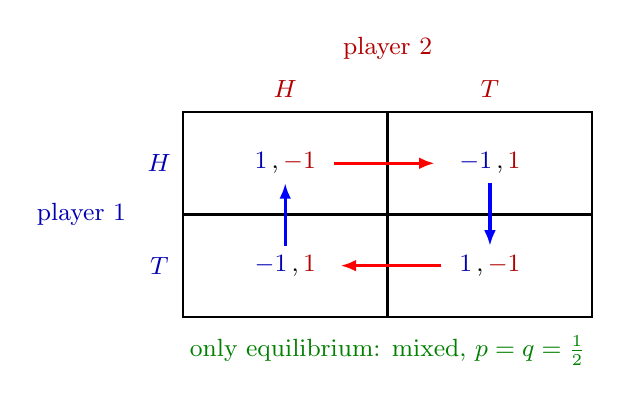
\begin{tikzpicture}[font=\small, >={Latex[length=2mm]}]
  \def\w{2.6} \def\h{1.3}
  \draw[thick] (0,-\h) rectangle (2*\w,\h);
  \draw[thick] (\w,-\h) -- (\w,\h);
  \draw[thick] (0,0) -- (2*\w,0);
  % strategy labels
  \node[red!70!black] at (0.5*\w,\h+0.3) {$H$};
  \node[red!70!black] at (1.5*\w,\h+0.3) {$T$};
  \node[blue!70!black] at (-0.3,0.5*\h) {$H$};
  \node[blue!70!black] at (-0.3,-0.5*\h) {$T$};
  \node[red!70!black, anchor=south] at (\w,\h+0.55) {player 2};
  \node[blue!70!black, anchor=east] at (-0.6,0) {player 1};
  % payoffs
  \node at (0.5*\w,0.5*\h) {\textcolor{blue!70!black}{$1$}\,,\,\textcolor{red!70!black}{$-1$}};
  \node at (1.5*\w,0.5*\h) {\textcolor{blue!70!black}{$-1$}\,,\,\textcolor{red!70!black}{$1$}};
  \node at (0.5*\w,-0.5*\h) {\textcolor{blue!70!black}{$-1$}\,,\,\textcolor{red!70!black}{$1$}};
  \node at (1.5*\w,-0.5*\h) {\textcolor{blue!70!black}{$1$}\,,\,\textcolor{red!70!black}{$-1$}};
  % deviation cycle
  \draw[->, very thick, red] (0.5*\w+0.62,0.5*\h) -- (1.5*\w-0.7,0.5*\h);
  \draw[->, very thick, blue] (1.5*\w,0.5*\h-0.25) -- (1.5*\w,-0.5*\h+0.25);
  \draw[->, very thick, red] (1.5*\w-0.62,-0.5*\h) -- (0.5*\w+0.7,-0.5*\h);
  \draw[->, very thick, blue] (0.5*\w,-0.5*\h+0.25) -- (0.5*\w,0.5*\h-0.25);
  \node[green!50!black, anchor=north] at (\w,-\h-0.12) {only equilibrium: mixed, $p=q=\tfrac{1}{2}$};
\end{tikzpicture}
\end{document}
